\documentclass[conference]{IEEEtran}
\usepackage[latin9]{inputenc}
\pagestyle{headings}
\usepackage{amsmath,amssymb}
\usepackage{graphicx,epsfig}
\usepackage{mathptmx,times} % if new font selection scheme installed
\usepackage{epstopdf}
\usepackage{tikz}
\usepackage[europeanresistors,americaninductors]{circuitikz}
\usepackage{mathtools}
\makeatletter
%%%%%%%%%%%%%%%%%%%%%%%%%%%%%% User specified LaTeX commands.
\hyphenation{op-tical net-works semi-conduc-tor}

\newcommand{\MYfooter}{\smash{
\hfil\parbox[t][\height][t]{\textwidth}{}\hfil\hbox{}}}

\def\ps@IEEEtitlepagestyle{%
\def\@oddhead{\mbox{}2016 ICSEE International Conference on the
     Science of Electrical Engineering \rightmark \hfil }%
\def\@oddfoot{\MYfooter}%
\def\@evenfoot{\MYfooter}}

% adjust as needed
\addtolength{\footskip}{0\baselineskip}
\addtolength{\textheight}{-1\baselineskip}

%%%%%%%%%%**********%%%%%%%%%%**********%%%%%%%%%%**********%%%%%%%%%%
\newtheorem{theorem}{Theorem}[section]
\newtheorem{corollary}[theorem]{Corollary}
\newtheorem{lemma}[theorem]{Lemma}

\newtheorem{proposition}[theorem]{Proposition}
\newtheorem{definition}[theorem]{Definition}
\newtheorem{example}[theorem]{Example}
\newtheorem{problem_statement}[theorem]{Problem Statement}
\newtheorem{remark}[theorem]{Remark}
%\numberwithin{equation}{section}
%%% The above 7 commands are used in the following way:
%%% The definition environment, for example, is created by
%%% \begin{definition}\label{xxx}. . .\end{definition}
%\newcommand{\mylabel}[1]{\label{#1}
%            \ifx\undefined\stillediting
%            \else \fbox{$#1$}\fi }
\newcommand{\BE}{\begin{equation}}
\newcommand{\BEQ}[1]{\BE\label{#1}} % Changed by Olof
\newcommand{\EEQ}{\end{equation}}
\newcommand{\rfb}[1]{\mbox{\rm
   (\ref{#1})}\ifx\undefined\stillediting\else:\fbox{$#1$}\fi}
\newenvironment{matr}[1]{\left[ \begin{array}{#1}}{\end{array}
                         \right]}
%
%\newfont{\roma}{cmr10 scaled 1200}
%\font\fourteenrm = cmr10  scaled\magstep2
%
\renewcommand{\cline}{{\mathbb C}}
\newcommand{\rline}  {{\mathbb R}}
\renewcommand{\l}    {{\lambda}}
\renewcommand{\o}    {{\omega}}
\newcommand{\e}      {{\varepsilon}}
\newcommand{\half}   {{\frac{1}{2}}}
\newcommand{\m}      {{\hbox{\hskip 1pt}}}
\newcommand{\nm}     {{\hbox{\hskip -3pt}}}
\newcommand{\dd}     {{\rm d\hbox{\hskip 0.5pt}}}

\makeatother

%%%%%%%%%%**********%%%%%%%%%%**********%%%%%%%%%%**********%%%%%%%%%%
\begin{document}

\title{ Exponential stability  of a microgid comprising of two identical synchronous generators}
\author{\IEEEauthorblockN{Elad Venezian} \IEEEauthorblockA{School of 
   EE, Tel Aviv University\\ Ramat Aviv 69978, Israel} \and 
   \IEEEauthorblockN{George Weiss} \IEEEauthorblockA{School of EE, 
   Tel Aviv University\\ Ramat Aviv 69978, Israel}}

\maketitle

\begin{abstract}
Synchronous generators are an essential component of the electric
grid. Recently, the stability of the electric grid has become an area
of high interest and intensive research. We discuss the stability of a
grid composed of two identical synchronous generators, and show sufficient conditions for exponential stability.
\end{abstract}

%%%%%%%%%%**********%%%%%%%%%%**********%%%%%%%%%%**********%%%%%%%%%%
\section{Introduction}

The AC electricity grid was developed at the end of the XIXth century,
and has remained very similar until today. The grid is an enormously
complex nonlinear and randomly varying system for which rigorous
stability analysis is impossible. Many techniques and models that have
been developed to assess the stability of a power grid, using rigorous
modelling and system theory techniques mixed with practical shortcuts
and simplifying assumptions driven by experience, see for instance
\cite{Kundur}, \cite{GrSt2014}, \cite{SauerPai1998}, \cite{GOBS:03},
\cite{DoBull:12}.

In recent years, due to the increasing penetration of renewable energy
resources, which connect to the grid via power converters and produce
an intermittent power output, it is not clear whether the traditional
models and methods for controlling the power grid will succeed to
control it. Therefore, there is an increasing interest in the
fundamental mathematical models and stability analysis for the grid,
see for instance \cite{DoBull:12}, \cite{PoDoBu:13}, \cite{CaTa:14},
\cite{NaWe:14}, \cite{NaWe:15}, \cite{DePersiSchaft:16}.

The {\em synchronous generator} (SG) is the main power source of the
electricity grid. The mathematical model of a SG (see the earlier
references and in addition \cite{Walker:94}, \cite{Fitzgerald:03},
\cite{MaWe:15}, etc.) is complex and difficult to use as a component
when we model a large network. Stability analysis is usually done
either by simulation, or analytically on simplified models, in which
the SGs are connected in a simple network and each SG is represented
by reduced order equations, see for instance \cite{DoBull:12} and
\cite{PoDoBu:13}. The reduced model of a SG is often obtained by
treating the stator currents as fast variables, thus eliminating them
from the state variables via the singular perturbation approach (see,
for instance, \cite{Khalil}) and keeping only the rotor angle, the
rotor angular velocity and the rotor field as relevant state
variables, see for instance \cite{Kundur} and \cite{SauerPai1998}.

SGs have the important property that once they synchronize, they tend
to remain synchronized even without any control. This is important
attribute because the electricity grid must maintain nearly constant
frequency, and because the ability of a SG to transfer constant power
to the grid exists only when the phase difference between it and the
grid is constant. Therefore, it is desirable to know if for a given
grid which contains SGs and a loads, the SGs tend to synchronize (for
initial states in a reasonably large region) and if yes, if the grid
frequency and power flows remains stable. To simplify the stability
analysis, it is common to use the Park transformation of the voltages
and currents, that maps sinusoidal positive sequence signals into a
fixed point in the state space.

In this paper, we study the configuration of a two identical SGs in parallel and a resistive  load. 

The rest of this paper is organized as follows. In Section II, a
fourth order model of a SG connected to infinite bus and having
constant field current is presented. The model of {\em two identical coupled SGs} (TICSG) is described in Section III. In section IV, we discuss  the equilibrium points of the TICSG system.
Stability analysis for the TICSG is given in Section IV.

%%%%%%%%%%**********%%%%%%%%%%**********%%%%%%%%%%**********%%%%%%%%%%
\section{Modeling SG connected to infinite bus}

In this section we derive the equations for a SG connected to infinite
bus and having a constant field (or rotor) current. We derive the equations for single SG, assuming constant field current,
following the notation in \cite{ZhWe:11}. 

The rotor of a SG is a winding (coil) on a magnetic core that spins
inside a circular cavity in the stator, having an angle $\theta$ with
respect to a reference angle, see Figure 1. We denote its self
inductance by $L_f$, its resistance by $R_f$, the voltage across its
terminals by $v_f$ and the current through it (called the field
current) by $i_f$. We assume for simplicity that $L_f$ is independent
of $\theta$ and $i_f$. The stator consists of three identical windings
that are connected in a star, with phase shifts of $120^0$ (see again
Figure 1). We consider that there is no neutral connection and no
damper windings. The stator windings can be regarded as connected
coils with self inductance $L$, mutual inductance $-M$, and resistance
$R_s$ (the parameters $L_f,R_f,L,M,R_s$ are positive). We assume no
magnetic saturation effects in the iron core and no Eddy currents. The
stator terminals are labeled with the letters $a,b,c$ and the vector
of voltages on the stator terminals is denoted by $v=\left[v_a\ v_b\
v_c\right]^\top$. We denote by $v_s$ the voltage at the unconnected 
center of the star (see Figure 1) and $v^n=[v_s\ v_s\ v_s]^\top$.
We define the vectors
$$ \widetilde{\cos}\m\theta \m=\m \left[\begin{array}{c} \cos\left(
   \theta\right)\\ \cos\left(\theta-\frac{2\pi}{3}\right)\\
   \cos\left(\theta-\frac{4\pi}{3}\right) \end{array}\right] \m,\quad
   \widetilde{\sin}\m\theta \m= \left[\begin{array}{c} \sin\left(
   \theta\right)\\ \sin\left(\theta-\frac{2\pi}{3}\right)\\ \sin\left
   (\theta-\frac{4\pi}{3}\right) \end{array}\right] \m.$$
We denote the stator flux by $\Phi=\left[\Phi_a\ \Phi_b\ \Phi_c
\right]^\top$, the stator currents by $i=\left[i_a\ i_b\ i_c\right]
^\top$ and the rotor current by $i_f$. 

%%%%%%%%%%**********%%%%%%%%%%**********%%%%%%%%%%**********%%%%%%%%%%
\begin{figure}
\begin{centering}
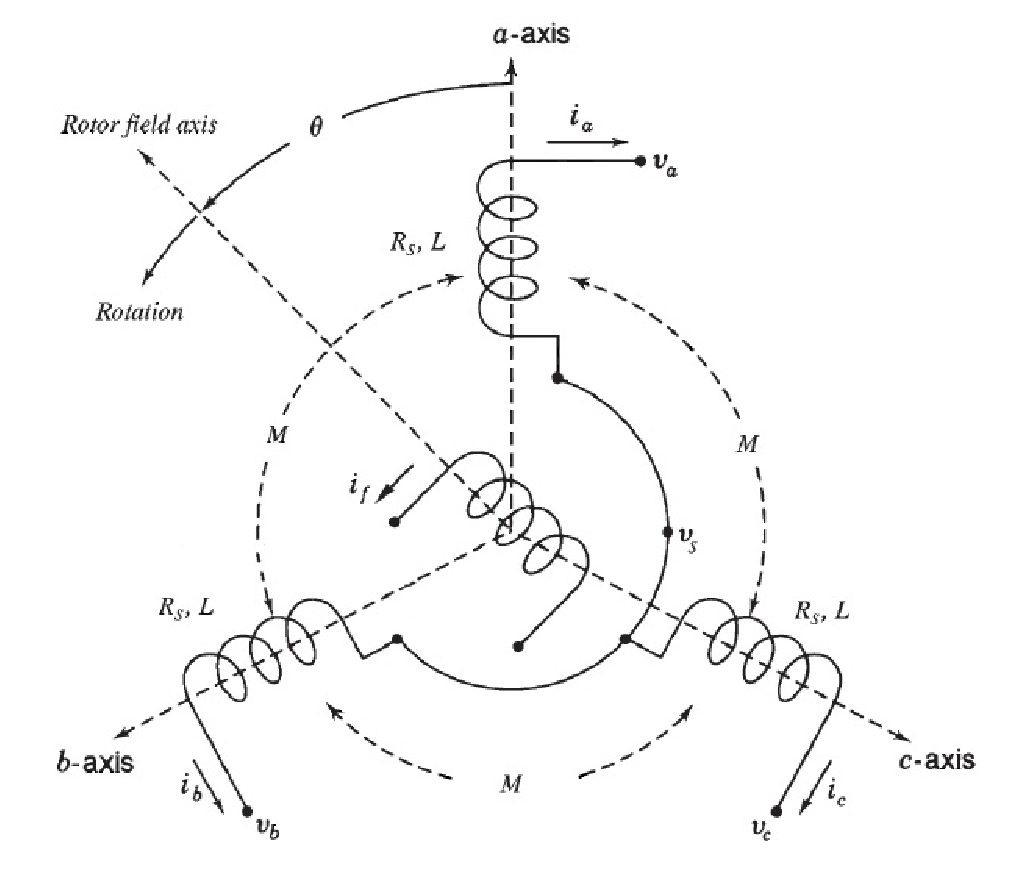
\includegraphics[scale=0.5]{SGStucture}
\par\end{centering} \label{fig:structOfSG}

\caption[Structure of an idealized three-phase round rotor synchronous
generator]{Structure of an idealized three-phase round rotor
synchronous generator, modified from \cite[Figure 3.4]{GrSt2014}.}
\end{figure}
%%%%%%%%%%**********%%%%%%%%%%**********%%%%%%%%%%**********%%%%%%%%%%

The mutual inductance between the rotor coil and each of the stator
coils varies with the rotor angle $\theta$ as follows:
$$ \left[\begin{array}{c} M_{a,f}\\ M_{b,f}\\ M_{c,f}\end{array}
   \right] \m=\m M_{f}\widetilde{\cos}\theta \m,$$
where $M_f>0$ is a constant. The vector of flux linkages of the stator
windings is
$$ \Phi \m=\m \left[\begin{array}{ccc} L & -M & -M\\ -M & L & -M\\
   -M & -M & L \end{array}\right]i + M_f i_f\widetilde{\cos}\theta
   \m.$$
Since there is no neutral line, $i_a+i_b+i_c=0$, so the previous
equation can be rewritten as 
$$\Phi \m=\m L_s i + M_f i_f \widetilde{\cos}\theta \m,$$
where $L_s=L+M$. We will assume that the rotor current is constant
(or equivalently, the rotor is composed of a permanent magnet). The
stator voltages satisfy
\BEQ{eq:SGTerminalVlotage}
   v - v^n \m=\m -R_{s}i-\frac{\dd\Phi}{\dd t} \m=\m -R_{s}i-L_{s}
   \frac{\dd i}{\dd t} + e \m,
\end{equation}
where $e=\left[e_a\ e_b\ e_c \right] ^\top$ is the back electromotive 
force (EMF) due to the rotor movement (also called synchronous 
internal voltage), given by \vspace{-2mm}
\BEQ{eq:emf}
   e \m=\m M_f i_f\dot{\theta}\widetilde{\sin}\theta \m.
\end{equation}

For a SG with no load, the voltages at each terminal
will be sinusoidal functions. In order to represent the voltages and
currents in a more convenient way, we apply the Park transformation
with respect to the rotor angle:
$$ x_{dq0} \m=\m \left[\begin{array}{c} x_{d}\\ x_{q}\\ x_{0}
   \end{array}\right] \m=\m U(\theta) \left[\begin{array}{c} x_{a}\\
   x_b\\ x_c\end{array}\right] \m=\m U(\theta) x_{abc} \m,$$
where $x_{abc}$ is a vector in $abc$ coordinates, $x_{dq0}$
is the same vector in the $dq0$ coordinates, and $U(\theta)$ is the
following unitary matrix:
\BEQ{eq:ParkTransformation}
 U(\theta) \m=\m \sqrt{\frac{3}{2}}\left[\begin{array}{ccc}
   \cos(\theta) & \cos(\theta-\frac{2\pi}{3}) & \cos(\theta-
   \frac{4\pi}{3})\\ \sin(\theta) & \sin(\theta-\frac{2\pi}{3})
   & \sin(\theta-\frac{4\pi}{3})\\ \sqrt{1/2} & \sqrt{1/2} & 
   \sqrt{1/2} \end{array}\right] \m.
\end{equation}

Applying the Park transformation to \rfb{eq:SGTerminalVlotage} 
leads to
\BEQ{aPark}
   U(\theta)(v-v^n)-U(\theta)e \m=\m -R_{s}U(\theta)i - L_s 
   U(\theta) \frac{\dd i}{\dd t} \m.
\end{equation}
Now we use that, denoting $i_{dq0}=U(\theta)i$,
$$ \frac{\dd i_{dq0}}{\dd\theta} \m=\m U(\theta)\frac{\dd i}
   {\dd\theta} + \frac{\dd U(\theta)}{\dd\theta}i \m=\m
   U(\theta)\frac{\dd i}{\dd\theta} + \left[\begin{array}{c}
   i_{q}\\ -i_{d}\\ 0 \end{array}\right].$$
This implies that \vspace{-2mm}
$$ \dot{i}_{dq0} \m=\m \frac{\dd i_{dq0}}{\dd\theta} \cdot \frac
   {\dd\theta}{\dd t} \m=\m U(\theta)\dot{i} + \o\left[\begin{array}
   {c} i_q\\ -i_d\\ 0 \end{array}\right] \m,$$
where $\o=\dot{\theta}$. We rewrite \rfb{aPark} as follows:
\BEQ{eq:idiqDynamics}
   L_s\frac{\dd}{\dd t}\nm\left[\nm\begin{array}{c} i_d\\ i_q\\ i_0
   \end{array}\nm\right] - L_s \o \left[\nm\begin{array}{c} i_q\\ -i_d
   \\ 0 \end{array}\nm\right] = -R_s\left[\begin{array}{c} i_d\\
   i_q\\ i_0 \end{array}\right] + \left[\nm \begin{array}{c} e_d-v_d
   \\ e_q-v_q\\ \tilde v\end{array}\nm\right],
\end{equation}
where $\tilde v=e_0-v_0+v^n_0$. Here we have used that (obviously)
$v^n_d=v^n_q=0$. Since there is no neutral connection, $i_0=0$, hence
$\tilde v=0$. Applying the Park transformation to \rfb{eq:emf} gives
$$ \left[\begin{array}{c} e_d\\ e_q \end{array}\right] \m=\m -\sqrt
   {\frac{3}{2}} M_{f} \left[ \begin{array}{c} 0\\ \o i_f
   \end{array}\right] \m.$$
We denote $m=\sqrt{\frac{3}{2}}M_{f}$. If we substitute the last
formula into \rfb{eq:idiqDynamics}, we get
\BEQ{eq:idiqDynamicsWithExIf}
   L_s\frac{\dd}{\dd t} \nm \left[\nm \begin{array}{c}
   i_d\\ i_q \end{array} \nm\right] = -R_s\left[\nm \begin{array}{c}
   i_d\\ i_q \end{array} \nm\right]+\o L_s\left[\nm\nm \begin{array}
   {c} i_q\\ -i_d\end{array} \nm\nm\right]\\ -m\left[\nm\nm 
   \begin{array}{c} 0\\ \o i_f\end{array} \nm\nm\right] - \left[\nm 
   \begin{array}{c} v_d\\ v_q \end{array} \nm\right] .
\end{equation}

The rotational dynamics of the rotor is given by
\BEQ{eq:mechanicalPart}
   J\dot{\omega} \m=\m T_{m}-T_{e}-D_{p} \omega \m,
\end{equation}
where $J$ is the moment of inertia of the rotor, $T_m-D_p\o$ is is the
mechanical torque coming from the prime mover, $T_e$ is the
electromagnetic torque developed by the generator, and $D_p$ is a the
frequency droop coefficient. The feedback term $D_p\o$ is used in
order to control the frequency of the grid, see \cite{Kundur},
\cite{PoDoBu:13}, \cite{CaTa:14}, \cite{ZhWe:11}. $T_e$ can be found
using energy consideration. It is easy to see that the magnetic 
energy stored in the generator is
$$ E_{mag} \m=\m \half \left(\langle i,L_s i \rangle + L_f i_f^2
   \right) + M_f i_f \langle i,\widetilde{\cos}\theta \rangle \m.$$
The electromagnetic torque can be calculated as follows:
$$ T_e \m=\m \frac{\partial E_{mag}}{\partial\theta}|_{\Phi,\Phi_f
   \ const.} \m=\m - \frac{\partial E_{mag}}{\partial\theta}|_{i,
   i_f\ const.}$$
(see \cite{ZhWe:11}), whence
$$ T_e \m=\m M_f i_f \left\langle i,\frac{\dd\tilde{\cos}\theta}
   {\dd\theta} \right\rangle \m=\m M_f i_f \langle i,\widetilde
   {\sin} \theta\rangle \m=\m -m i_f i_q \m.$$
Using \rfb{eq:idiqDynamicsWithExIf}, \rfb{eq:mechanicalPart}
and the last formula, we obtain
\BEQ{eq:SingleSGDynamics}
   \frac{\dd}{\dd t}\nm\left[\nm \begin{array}{c} L_s i_d\\ L_s i_q\\ 
   J\o\end{array} \nm\right] = \left[\nm \begin{array}{ccc} -R_s & 
   \o L_s & 0\\ -\o L_s & -R_s & -mi_f\\ 0 & mi_f & -D_p \end{array}
   \nm\right] \nm \left[\nm \begin{array}{c} i_d\\ i_q\\ \o 
   \end{array} \nm\right] + \left[\nm\nm \begin{array}{c} -v_d\\ -v_q
   \\ T_m \end{array} \nm\nm\right].
\end{equation}
This third order nonlinear dynamical system represents the dynamics
of a single SG with constant field current, if we ignore the rotor 
angle $\theta$. 

\section{TICSG modeling}

In this section we develop a model for a microgid comprising of two identical SGs connected in parallel with a resistive load, assuming constant field current (see Figure \ref{fig:TICSGThreePhase}).

%%%% Figure Tree phase TICSG system.
\begin{figure}[!htb]
\begin{circuitikz}[american voltages,scale=0.6, transform shape]
\begin{scope}[shift={(-5,0)}]     \draw (0,0) node[anchor=east] {0} to [L=Z, *-o] (90 :2.5) node[anchor=east]{$v_a$}; \draw (0,0) to [L=Z, *-o] (210 :2.5) node[anchor=east]{$v_b$}; \draw (0,0) to [L=Z, *-o] (330 :2.5) node[anchor=east]{$v_c$}; \node (0,0) [align=left,text width=4cm] {SG1}; \end{scope}
   \draw (0,0) node[anchor=east] {0} to [R=$R_L$, *-o] (90 :2.5) node[anchor=east]{}; \draw (0,0) to [R=$R_L$] (210 :2.5); \draw (0,0) to [R=$R_L$] (330 :2.5);
\begin{scope}[shift={(5,0)}]    \draw (0,0) node[anchor=east] {0} to [L=Z, *-o] (90 :2.5) node[anchor=west] {$v_a$}; \draw (0,0) to [L=Z, *-o] (210 :2.5) node[anchor=east]{$v_b$}; \draw (0,0) to [L=Z, *-o] (330 :2.5) node[anchor=east]{$v_c$}; \node (0,0) [align=left,text width=4cm] {SG2}; \end{scope}
\draw (5,2.5) to [short, i>=$i_{a2}$] (0,2.5) to [short, i<=$i_{a1}$] (-5,2.5); \draw (-2.165 +5,-1.25) to [short] (-2.165 +5,-1.25 -1) to [short, i>=$i_{b2}$]   (-2.165 ,-1.25-1)  to [short, o-] (-2.165 ,-1.25 ); \draw (-2.165 -5,-1.25) to [short] (-2.165 -5,-1.25 -1) to [short, i>=$i_{b1}$]   (-2.165 ,-1.25-1); \draw (2.165 +5,-1.25) to [short] (2.165 +5,-1.25 -2) to [short, i>=$i_{c2}$]  (2.165 ,-1.25-2)  to [short, o-] (2.165 ,-1.25 ); \draw (2.165 -5,-1.25) to [short] (2.165 -5,-1.25 -2) to [short, i>=$i_{c1}$]  (2.165 ,-1.25-2);
\end{circuitikz}\caption{{\em two identical coupled SGs} (TICSG) model - three phase diagram}

\label{fig:TICSGThreePhase}
\end{figure}

%%%%%%%%%%%%%
We denote the first SG rotor angle as  $\theta_{1}$ and the second SG rotor angle as $\theta_{2}$. We assume identical constant torque that act on each of the generators, denoted as $T_{m}$. By symmetry,
we assume that the voltages at the (non-connected) midpoints of the
generators and the load are zero.

We denoted the phase voltages and currents of the first generator as: $v_{1}=\left[v_{a1}\  v_{b1}\  v_{c1}
\right]^\top$ and $i_{1}=\left[i_{a1}\  i_{b1}\  i_{c1}
\right]^\top$  respectively.
Similarly, we denoted the phase voltages and currents of the second generator as: $v_{2}=\left[v_{a2}\  v_{b2}\  v_{c2}
\right]^\top$ and $i_{2}=\left[i_{a2}\  i_{b2}\  i_{c2}
\right]^\top$ respectively.

We denote by $Z$ the impedance of each SG stator. This impedance is comprised by the resistive impedance of the stator coil $R_s$ and the inductive impedance of the stator, namely $Z\left(s\right)=R_{s} + sL_{s}$. In general, the line that connects the SG to the grid has its impedance that can be modeled (in most cases) as a resistance and an inductance in series, but these values can simply be added to the parameters $R_s$ and $L_s$ of the SG.
One phase scheme of the grid is presented at Figure \ref{fig:TICSGOnePhase}.


%%%% Figure Tree phase TICSG system.
\begin{figure}[!htb]
\begin{circuitikz}[american voltages,scale=0.6, transform shape]
\draw   (0,0) node[ground] {}   to [V,v=$e_{j1}$] (0,3) {}   to [R=$R_s$,i>=$i_{j1}$] (3,3){}   to [L=$L_s$] (5,3){}   to [R=$R_L$, o-] (5,0){}    to  (5,0) node[ground] {};   \draw   (10,0) node[ground] {}   to [V,v=$e_{j2}$] (10,3) {}   to [R=$R_s$,i>=$i_{j2}$] (7,3){}   to [L=$L_s$] (5,3){};   \node[draw] at (-1,4) {$j \in \{a,b,c\}$}; \end{circuitikz} 

\caption{{\em two identical coupled SGs} (TICSG) model - one phase diagram}

\label{fig:TICSGOnePhase}
\end{figure}

%%%%%%%%%

In order to use the fourth order model of a single SG \eqref{eq:SingleSGDynamics} in the two SGs system, we apply  the Park transformation \eqref{eq:ParkTransformation}, on each SG  terminal voltages: $\left[ v_{di}\ v_{qi}\  v_{0i} \right]^\top=U(\theta_{i})\left[v_{ai}\ v_{bi}\ v_{ci}  \right]^\top$,  and currents $\left[v_{di}\ v_{qi}\  v_{0i} \right]^\top=U(\theta_{i})\left[v_{ai}\ v_{bi}\ v_{ci}  \right]^\top$,  ($i \in \{1,2\}$).

An expression of the voltage at each SG terminal is:
$$v_1=v_2=R_{L}(i_{1}+i_{2})$$

Rewriting this equation for the first SG after applying Park transformation yields:

$$
\left[\begin{array}{c}
v_{d1}\\
v_{q1}\\
v_{01}
\end{array}\right]=R_{L}\left[\begin{array}{c}
i_{d1}\\
i_{q1}\\
i_{01}
\end{array}\right]+R_{L}U(\theta_{1})\left[\begin{array}{c}
i_{a2}\\
i_{b2}\\
i_{c2}
\end{array}\right]
$$

Because Park transformations argument is  $\theta_1$,  the second SG current can't be transformed directly to the d-q coordinates:   $U(\theta_{1})\left[ i_{a2}\ i_{b2}\ i_{c2}\right]^\top \neq \left[ i_{d2}\ i_{q2}\ i_{02}\right]$. 

We express  the currents of the second SG in the d-q coordinates by using the inverse Park transformation: 
\BEQ{eq:TICSGVolAndCurr}
 \left[\begin{array}{c}
v_{d1}\\
v_{q1}\\
v_{01}
\end{array}\right]=R_{L}\left[\begin{array}{c}
i_{d1}\\
i_{q1}\\
i_{01}
\end{array}\right]+R_{L}U(\theta_{1})U(\theta_{2})^{-1}\left[\begin{array}{c}
i_{d2}\\
i_{q2}\\
i_{02}
\end{array}\right].
\end{equation}

We denote $$\delta=\theta_{2}-\theta_{1}$$

A simple computation shows that 
\BEQ{eq:ParkChangeAngle}
  U(\theta_{1})U(\theta_{2})^{-1}=\left[\begin{array}{ccc}
\cos(\delta) & -\sin(\delta) & 0\\
\sin(\delta) & \cos(\delta) & 0\\
0 & 0 & 1
\end{array}\right].
\end{equation}

Because our assumption that the SGs don't have a neutral connection, and by using Kirchhoff's laws we obtain that $i_{01}=i_{02}=0$.  Substituting this into \eqref{eq:TICSGVolAndCurr} and \eqref{eq:ParkChangeAngle} shows that $v_{01} = 0$.

Substitute \eqref{eq:SingleSGDynamics} and \eqref{eq:ParkChangeAngle} into \eqref{eq:TICSGVolAndCurr}  gives:

\[
\varLambda\dot{z}_{1}=\mathcal{A}(\omega_{1})z_{1}+T_{m}e_{3}-\mathcal{B}(\delta)z_{2}
\]
Where we denote
 \[z_{i}=\left[i_{di}\ i_{qi}\  \omega_{i}\right]^\top,i\in\{1,2\},\]

\[
\varLambda=\left[\begin{array}{ccc}
L_{s} & 0 & 0\\
0 & L_{s} & 0\\
0 & 0 & J
\end{array}\right],
\]

\[
\mathcal{A}(\omega)=\left[\begin{array}{ccc}
-R_{tot} & \omega L_{s} & 0\\
-\omega L_{s} & -R_{tot} & -mi_{f}\\
0 & mi_{f} & D_{p}
\end{array}\right],
\]
\[\mathcal{B}(\delta)=\left[\begin{array}{ccc}
R_{L}\cos(\delta) & -R_{L}\sin(\delta) & 0\\
R_{L}\sin(\delta) & R_{L}\cos(\delta) & 0\\
0 & 0 & 0
\end{array}\right],
\]
\[e_{3}=\left[0\ 0\ 1\right]^\top\] and
\[ R_{tot}=R_{s}+R_{L} \]

Of course a symmetric equation holds for the second generator:

\[
\varLambda\dot{z}_{2}=\mathcal{A}(\omega_{2})z_{2}+T_{m}e_{3}-\mathcal{B}(-\delta)z_{1}
\]

We denote the angular velocity  of the SG rotor as $\omega_i = \dot{\theta_i}$ where $i \in \{1,2\}$. 
An additional ODE for $\delta$ is:

\[
\dot{\delta}=\omega_{2}-\omega_{1}
\]

Rewriting the entire system dynamics gives:

\begin{equation}
\begin{array}{ccc}
\frac{d}{dt}\left[\begin{array}{c}
\varLambda z_{1}\\
\varLambda z_{2}\\
\delta
\end{array}\right] & = & \left[\begin{array}{c|c|c}
\mathcal{A}(\omega_{1}) & -\mathcal{B}(\delta) & 0\\
\hline -\mathcal{B}(-\delta) & \mathcal{A}(\omega_{2}) & 0\\
\hline -e_{3}^{T} & e_{3}^{T} & 0
\end{array}\right]\left[\begin{array}{c}
z_{1}\\
z_{2}\\
\delta
\end{array}\right]\\
 &  & +T_{m}\left[\begin{array}{c}
e_{3}\\
e_{3}\\
0
\end{array}\right]
\end{array}\label{eq:TICSGDynamics}
\end{equation}

We refer this seven order non linear dynamic system as the TICSG model.
%%%%%%%%%%**********%%%%%%%%%%**********%%%%%%%%%%**********%%%%%%%%%%

\section{Analysis of the equilibrium points of the TICSG model \label{sec:equivalence_pont}}

In this section, we study the equilibrium points of the TICSG system. First, we show that  if there exist equilibrium points, they must located on the synchronization subspace or on the anti-synchronization subspace i.e. any equilibrium point $\left[z_1^e \ z_2^e \ \delta^e \right]^\top$ must satisfy $z_1^e=z_2^e$ and $\delta^e=0$ or $\delta^e = \pi$   (modulo $2\pi$). Second, we show that the TICSG system has at list one equilibrium point on the synchronization subspace (i.e with $\delta^e=0$).

\subsection{An equilibrium point must satisfy synchronization condition.}
We  start by investigate the solution of the algebraic equation:  

\begin{equation}
\left[\begin{array}{c|c|c}
\mathcal{A}(\omega_{1}^{e}) & -\mathcal{B}(\delta^{e}) & 0\\
\hline -\mathcal{B}(-\delta^{e}) & \mathcal{A}(\omega_{2}^{e}) & 0\\
\hline -e_{3}^{T} & e_{3}^{T} & 0
\end{array}\right]\left[\begin{array}{c}
z_{1}^{e}\\
z_{2}^{e}\\
\delta^{e}
\end{array}\right]+T_{m}\left[\begin{array}{c}
e_{3}\\
e_{3}\\
0
\end{array}\right]=0
\label{eq:algebricEquation}
\end{equation}

It easy to see that according to the seventh line $$\omega_{1}^{e}=\omega_{2}^{e}=\omega^{e}$$.

From the third and the sixth lines we have: 

$$
\left\{ \begin{array}{c}
mi_{f}i_{q1}^{e}-D_{p}\omega_{1}^{e}+T_{m}=0\\
mi_{f}i_{q2}^{e}-D_{p}\omega_{2}^{e}+T_{m}=0
\end{array}\right.\longrightarrow i_{q1}^{e}=i_{q2}^{e}=i_{q}^{e}
$$

From the first, second, fourth and fifth lines:

$$
 \begin{array}{c}
-R_{tot}i_{d1}^{e}+\omega^{e}L_{s}i_{q}^{e}-R_{L}\cos\delta^{e}i_{d2}^{e}+R_{L}\sin\delta^{e}i_{q}^{e}=0\\
-\omega^{e}L_{s}i_{d1}^{e}-R_{tot}i_{q}^{e}-mi_{f}\omega^{e}-R_{L}\sin\delta^{e}i_{d2}^{e}-R_{L}\cos\delta^{e}i_{q}^{e}=0\\
-R_{tot}i_{d2}^{e}+\omega^{e}L_{s}i_{q}^{e}-R_{L}\cos\delta^{e}i_{d1}^{e}-R_{L}\sin\delta^{e}i_{q}^{e}=0\\
-\omega^{e}L_{s}i_{d2}^{e}-R_{tot}i_{q}^{e}-mi_{f}\omega^{e}+R_{L}\sin\delta^{e}i_{d1}^{e}-R_{L}\cos\delta^{e}i_{q}^{e}=0
\end{array}
$$
By denoting:
\[
M=\left[\begin{array}{cc}
-R_{tot} & -R_{L}\cos\delta^{e}\\
-\omega^{e}L_{s} & -R_{L}\sin\delta^{e}\\
-R_{L}\cos\delta^{e} & -R_{tot}\\
R_{L}\sin\delta^{e} & -\omega^{e}L_{s}
\end{array}\right]
\]

and 

\[
n=\left[\begin{array}{c}
i_{q}^{e}\left(\omega^{e}L_{s}+R_{L}\sin\delta^{e}\right)\\
-mi_{f}\omega^{e}-i_{q}^{e}\left(R_{tot}+R_{L}\cos\delta^{e}\right)\\
i_{q}^{e}\left(\omega^{e}L_{s}-R_{L}\sin\delta^{e}\right)\\
-mi_{f}\omega^{e}-i_{q}^{e}\left(R_{tot}+R_{L}\cos\delta^{e}\right)
\end{array}\right]
\]
We represent these lines in the following way:

\begin{equation}
M\left[\begin{array}{c}
i_{d1}^{e}\\
i_{d2}^{e}
\end{array}\right]=n\label{eq:equilibrium_system}
\end{equation}

Now, we  show by contradiction that any equilibrium point must satisfy: $\sin\delta^e=0$.
We use Rouch\'e Capelli Theorem:  Any liner equations system with the form  $Mx=n$ has a  solution if and only if $rank\left[M|n\right]=rank\left[M\right].$

We negated to assume that $\sin\delta^{e}\ne0$. Simple calculation shows that under this assumption   $rank\left[M|n\right]=3$ must hold.

Obviously, $rank\left[M\right]\le2$.  Rouch\'e Capelli Theorem implies that under the
previous assumption the linear equations system \eqref{eq:equilibrium_system} doesn't have solution. It proves that  if the TICSG system has an equilibrium point, it must satisfied: $\sin\delta^{e}=0$ means that : $\delta^{e}=0$ or $\delta^e = \pi$ (modulo $2\pi$).

After subtitling $\sin\delta^{e}=0$
and $\cos\delta^{e}=\pm 1$, the linear equations system  \eqref{eq:equilibrium_system} becomes:

$$
M=\left[\begin{array}{cc}
-R_{tot} & \mp R_{L}\\
-\omega^{e}L_{s} & 0\\
  \mp R_{L} & -R_{tot}\\
0 & -\omega^{e}L_{s}
\end{array}\right]
$$

and 

$$
N=\left[\begin{array}{c}
i_{q}^{e}\omega^{e}L_{s}\\
-mi_{f}\omega^{e}-i_{q}^{e}\left(R_{tot} \pm R_{L}\right)\\
i_{q}^{e}\omega^{e}L_{s}\\
-mi_{f}\omega^{e}-i_{q}^{e}\left(R_{tot} \pm R_{L}\right)
\end{array}\right]
$$

This solution of this system is: $i_{d1}^{e}=i_{d2}^{e}$.



\subsection{The TICSG system has at list one equilibrium point on the synchronization subspace}
Here, we show that the TICSG system has at list one equilibrium point which satisfies 
\begin{equation}
z_1^{e}=z_2^{e}=z^{e},\quad \delta^e=0\label{eq:eqPointConditions}
\end{equation}

After substituting condition \eqref{eq:eqPointConditions} into \eqref{eq:algebricEquation} ,we get:

\begin{equation}
\left[\begin{array}{ccc}
-R_{s}-2R_{L} & \omega^{e}L_{s} & 0\\
-\omega^{e}L_{s} & -R_{s}-2R_{L} & -mi_{f}\\
0 & mi_{f} & -D_{p}
\end{array}\right]\left[\begin{array}{c}
i_{d}^{e}\\
i_{q}^{e}\\
\omega^{e}
\end{array}\right]=\left[\begin{array}{c}
0\\
0\\
-T_{m}
\end{array}\right]\label{eq:equilbrium_algebric_eq}
\end{equation}

We take scalar products on both sides with $z^{e}$:

\[
\left(R_{tot}+R_{L}\right)\left((i_{d}^{e})^{2}+(i_{q}^{e})^{2}\right)=\left(T_{m}-D_{p}\omega^{e}\right)\omega^{e}
\]

This equation makes perfect physical sense. Indeed, assume that there
is no actual friction in the machine, $D_{p}$ is created by feedback,
so that $T_{m}-D_{p}\omega^{e}$ is the mechanical torque applied
to one generator, and then $\left(T_{m}-D_{p}\omega^{e}\right)\omega^{e}$
is the mechanical power entering one generator. On the other hand,
it is easy to see that $\left(R_{tot}+R_{L}\right)\left((i_{d}^{e})^{2}+(i_{q}^{e})^{2}\right)=\left(R_{s}+2R_{L}\right)\left(i_{a}^{2}+i_{b}^{2}+i_{c}^{2}\right)$
which is exactly half of the power dissipated in all the resistors,
hence it is the electric power leaving one generator.

From \eqref{eq:equilbrium_algebric_eq}, we derive a scalar
equation to determine the equilibrium velocity $\omega^{e}$.
From the last line of the matrix equation\eqref{eq:equilbrium_algebric_eq} we have

\begin{equation}
T_{m}-D_{p}\omega^{e}=-mi_{f}i_{q}^{e}\label{eq:eq_0_first_eq}
\end{equation}

The left side of this equation can interpreted as the  mechanical torque acting on each
generator at equilibrium.

The first line of the matrix equilibrium \eqref{eq:equilbrium_algebric_eq}
is $-\left(R_{tot}+R_{L}\right)i_{d}^{e}+\omega^{e}L_{tot}i_{q}^{e}=0$,
hence:

\[
i_{d}^{e}=\frac{\omega^{e}L_{s}}{R_{tot}+R_{L}}i_{q}^{e}
\]

From \eqref{eq:eq_0_first_eq} 
\begin{equation}
i_{q}^{e}=\frac{T_{m}-D_{p}\omega^{e}}{-mi_{f}}\label{eq:iq_0_}
\end{equation}

Combining the last two formulas,

\begin{equation}
i_{d}^{e}=-\frac{\omega^{e}L_{s}}{R_{tot}+R_{L}}\frac{T_{m}-D_{p}\omega^{e}}{mi_{f}}\label{eq:id_0_}
\end{equation}

The second line of the matrix equation on \eqref{eq:eq_0_first_eq},
is 
$$\omega^{e}L_{s}i_{d}^{e}+\left(R_{tot}+R_{L}\right)i_{q}^{e}+mi_{f}\omega^{e}=0$$
Substituting in this equation the expressions for ,$i_{q}^{e}$ and $i_{d}^{e}$ yields the following cubic equation in $\omega^e$, denoting $R_T = R_L+R_{tot}$:

\begin{equation}
\begin{split}
D_{p}L_{s}^{2}\left(\omega^{e}\right)^{3}-T_{m}L_{s}^{2}\left(\omega^{e}\right)^{2} +\left(D_{p}R_T^{2}+m^{2}i_{f}^{2}R_T\right) \omega^{e}  -T_{m}R_T^{2}=0
\end{split}\label{eq:cuibi_eq}
\end{equation}

Let us denote the polynomial of order 3 in \eqref{eq:cuibi_eq} by
$p(\omega^{e})$. 
$$p(0)=-T_{m}R_T^{2}<0$$
On the other hand, we note that 
$$
p(\frac{T_{m}}{D_{p}}) =m^{2}i_{f}^{2}R_T\frac{T_{m}}{D_{p}}>0
$$

Hence, \eqref{eq:cuibi_eq} has at least one solution in the interval
$\omega^{e}\in\left(0,\frac{T_{m}}{D_{p}}\right)$.

That shows that the TICSG system has at list one equilibrium point  that located on the synchronization subspace 
$\epsilon=\{ \left[z^e \ z^e \ \delta^e  \right]^\top   |  \delta^e= 0\}$.

Note, that the anti synchronization subspace  $\epsilon '=\{ \left[z^e \ z^e \ \delta^e  \right]^\top   |  \delta^e=\pi \}$ may also have equilibrium points.
%%%%%%%%%%**********%%%%%%%%%%**********%%%%%%%%%%**********%%%%%%%%%%

\section{Synchronization}

In this section, we show that the synchronization subspace of the TICSG system, is locally exponentially stable.
We start with rewrite the TICSG dynamics as synchronization error
 and equivalence SG dynamics. Then, we  prove that under
some conditions, the equivalence SG dynamics is globally exponentially
stable. Finally, we use the main result from  \cite{AndrieuJayawardhanaPraly},
to show the stability of the system near the synchronization subspace.

\subsection{Modeling the synchronization problem:}
The TICSG system has the following structure:
$$ \tilde{\Lambda}\frac{d}{dt}\left[z_1\ z_2\ \delta\right]^{\top}= f\left( \left[z_1\ z_2\ \delta\right]^{\top} \right)$$
where $\tilde{\Lambda} = diag \left( \Lambda,\Lambda,1 \right) $.
In order to show synchronization, it is convenient to denote:
$$e =  \left[\left(z_1^\top-z_2^\top \right)\ \delta \right]^\top = \left[e_d\ e_q\ e_{\omega}\ \delta \right]^\top $$
and 
$$x =z_1+z_2 = \left[ x_d\ x_q\ x_\omega\right]^\top.$$  

And to use the following structure:

\begin{equation}
\left\{ \begin{array}{c}
\dot{e}=F(e,x)\\
\dot{x}=G(e,x)
\end{array}\right.\label{eq:sync_sestem}
\end{equation}

For some functions $F$ and $G$. 

From \eqref{eq:TICSGDynamics}:
$$
\begin{aligned}
\Lambda(\dot{z}_{1}-\dot{z}_{2})&=\mathcal{A}(\omega_{1})z_{1}+T_{m}e_{3}-\mathcal{B}(\delta)z_{2}\\&-\left(\mathcal{A}(\omega_{2})z_{2}+T_{m}e_{3}-\mathcal{B}(-\delta)z_{1}\right)
\end{aligned}
$$
Calculating  $F$:
$$
\begin{aligned}
&  \left[\begin{array}{cc}
\varLambda & 0\\
0 & 1
\end{array}\right] \frac{d}{dt}\left[\begin{array}{c}
e_{d}\\
e_{q}\\
e_{\omega}\\
\delta
\end{array}\right]  =  \\ & \left[\begin{array}{c}
-R_{tot}(i_{d1}-i_{d2})+L_{s}(\omega_{1}i_{q1}-\omega_{2}i_{q2})\\
-L_{s}(\omega_{1}i_{d1}-\omega_{2}i_{d2})-R_{tot}(i_{q1}-i_{q2})-mi_{f}(\omega_{1}-\omega_{2})\\
mi_{f}(i_{q1}-i_{q2})-D_{p}(\omega_{1}-\omega_{2})\\
-(\omega_{1}-\omega_{2})
\end{array}\right]\\
 + & \left[\begin{array}{c}
R_{L}\cos(\delta)(i_{d1}-i_{d2})+R_{L}\sin(\delta)(i_{q1}+i_{q2})\\
R_{L}\cos(\delta)(i_{q1}-i_{q2})-R_{L}\sin(\delta)(i_{d1}+i_{d2})\\
0\\
0
\end{array}\right].
\end{aligned}
$$

Because the following equation   
$$(a+b)(x-y)+(a-b)(x+y)=2(ax-by)$$
holds for any $x$, $y$, $a$ and $b$, it implies that:
$$
\begin{aligned}
\omega_{1}i_{q1}-\omega_{2}i_{q2}= &\frac{1}{2}\left[(\omega_{1}+\omega_{2})(i_{q1}-i_{q2})+(\omega_{1}-\omega_{2})(i_{q1}+i_{q2})\right] \\ =&\frac{x_{w}e_{q}+e_{w}x_{q}}{2}
\end{aligned}
$$

and the previous equation can be rewritten as:
$$
\dot{e}  = F(e,x) =\left[\begin{array}{cc}
\varLambda & 0\\
0 & 1
\end{array}\right]^{-1}\left(A_e\left(x,e\right) e +B_e\left(x,e\right)  \right)
$$

Where 

$$
\begin{aligned}
&A_x\left(x,e\right)  = \\ & \left[\begin{array}{cccc}
-R_{tot}+R_{L}\cos\delta & \frac{L_{s}}{2}x_{\omega} & \frac{L_{s}}{2}x_{q} & 0\\
-\frac{L_{s}}{2}x_{\omega} & -R_{tot}+R_{L}\cos\delta & -\frac{L_{s}}{2}x_{q}-mif & 0\\
0 & mi_{f} & -D_{p} & 0\\
0 & 0 & -1 & 0
\end{array}\right]
\end{aligned}
$$ 
and
$$
B_x\left(x,e\right) = 
\left[\begin{array}{c}
R_{L}\sin(\delta)x_{2}\\
-R_{L}\sin(\delta)x_{1}\\
0\\
0
\end{array}\right].
$$



We note that $F(0,x)=0$, which shows that the subspace
$\epsilon=\left\{ \left[\begin{array}{c}
x\\
e
\end{array}\right]\in\mathbb{R}^{7}|e=0\right\} $ is invariant.

For the $x$ dynamics, we have:

$$
\begin{aligned}
\Lambda(\dot{z}_{1}+\dot{z}_{2})= & \mathcal{A}(\omega_{1})z_{1}+T_{m}e_{3}-\mathcal{B}(\delta)z_{2}\\+&\mathcal{A}(\omega_{2})z_{2}  +T_{m}e_{3}-\mathcal{B}(-\delta)z_{1}
\end{aligned}
$$

$$
\begin{aligned}
&\Lambda\frac{d}{dt}\left[\begin{array}{c}
x_{d}\\
x_{q}\\
x_{\omega}
\end{array}\right]  = \\
 & \left[\begin{array}{c}
-R_{tot}(i_{d1}+i_{d2})+L_{s}(\omega_{1}i_{q1}+\omega_{2}i_{q2})\\
-L_{s}(\omega_{1}i_{d1}+\omega_{2}i_{d2})-R_{tot}(i_{q1}+i_{q2})-mi_{f}(\omega_{1}+\omega_{2})\\
mi_{f}(i_{q1}+i_{q2})-D_{p}(\omega_{1}+\omega_{2})+2T_{m}
\end{array}\right]\\
 +& \left[\begin{array}{c}
-R_{L}\cos(\delta)(i_{d1}+i_{d2})-R_{L}\sin(\delta)(i_{q1}-i_{q2})\\
-R_{L}\cos(\delta)(i_{q1}+i_{q2})+R_{L}\sin(\delta)(i_{d1}-i_{d2})\\
0
\end{array}\right]
\end{aligned}
$$

Again, because the  equation  
$$
(a+b)(x+y)+(a-b)(x-y)=2(ax+by)
$$
holds for any $x$, $y$, $a$ and $b$, it implies that:
$$
\begin{aligned}
\omega_{1}i_{q1}+\omega_{2}i_{q2} &=\frac{1}{2}\left[(\omega_{1}+\omega_{2})(i_{q1}+i_{q2})+(\omega_{1}-\omega_{2})(i_{q1}-i_{q2})\right]\\ & =\frac{x_{w}x_{q}+e_{w}e_{q}}{2}
\end{aligned}
$$

and similarly:

$$
\omega_{1}i_{d1}-\omega_{2}i_{d2}=\frac{x_{w}x_{d}+e_{w}e_{d}}{2}
$$ 

And the $x$ dynamics can be rewrite as:
$$ \dot{x}=G \left( x,e\right)= \Lambda^{-1}\left(A_x \left(x,e \right) x + B_x \left( x,e\right) \right) $$

Where
$$
A_x \left(x,e \right)=\left[\begin{array}{ccc}
-R_{tot}-R_{L}\cos(\delta) & \frac{L_{s}}{2}x_{\omega} & 0\\
-\frac{L_{s}}{2}x_{\omega} & -R_{tot}-R_{L}\cos(\delta) & -mif\\
0 & mi_{f} & -D_{p}
\end{array}\right]
$$

$$
B_x \left(x,e \right)=\left[\begin{array}{c}
\frac{L_{s}}{2}e_{\omega}e_{q}-R_{L}\sin(\delta)e_{q}\\
-\frac{L_{s}}{2}e_{\omega}e_{d}-R_{L}\sin(\delta)e_{d}\\
2T_{m}
\end{array}\right]
$$

\subsection{Globally exponentially stability of the TICSG system on the synchronization subspace }

In this subsection, we provide sufficient conditions for the equilibrium
point which located on the synchronization subspace $\epsilon=\left\{ \left[ e\ x \right]^\top \in\mathbb{R}^{7}|e=0\right\} $,  to be a globally exponential stable equilibrium point, for trajectories with initial condition that lies on the $\epsilon$ subspace.  Because we showed that  $\epsilon$ is invariant subspace, it means that any trajectory that starts within this subspace, remains inside it.

We denote the state variables of of these trajectories as $\tilde{x} = \left[x_d \ x_q\ x_\omega \right]^\top$. 

The dynamics of these trajectories is (denoted as $\tilde{G}$):
$$
\dot{\tilde{x}}=\tilde{G}(\tilde{x})=G(0,\tilde{x})=
 \Lambda^{-1} A\left( \tilde{x}_\omega \right) \tilde{x}+\Lambda^{-1} B 
$$

Where we denote:
$$
A\left( \tilde{x}_\omega \right)=A_x\left(0, \tilde{x}_\omega \right) =  
 \left[\begin{array}{ccc}
-R_T & \frac{L_{s}}{2}\tilde{x}_{\omega} & 0\\
-\frac{L_{s}}{2}\tilde{x}_{\omega} & -R_T & -mif\\
0 & mi_{f} & -D_{p}
\end{array}\right]
$$
and
$$
B = B_x\left(0, \tilde{x}_\omega \right)  =  
 \left[\begin{array}{c}
0\\
0\\
2T_{m}
\end{array}\right].
$$

This system describes the two SGs with perfect synchronization between each other.

Because the TICSG system has at list one equilibrium point on the $\epsilon$ subspace, it means that $\tilde{G}(\tilde{x})$ has at list one equilibrium point 
$\tilde{x}^{e}=\left[\tilde{x}_{d}^{e}\ \tilde{x}_{q}^{e}\ \tilde{x}_{\omega}^{e} \right]^\top = 2z^e$ (recall that by definition $x = z_1 + z_2$).

\begin{equation}
\tilde{G}(\tilde{x}^{e})=0\rightarrow\varLambda^{-1}A(\tilde{x}_{\omega}^{e})\tilde{x}^{e}+\varLambda^{-1}\left[\begin{array}{c}
0\\
0\\
2T_{m}
\end{array}\right]=0\label{eq:G_at_equilibrium}
\end{equation}

In order to shift the equilibrium point into the origin, we denote the new  coordinates:
$$
\hat{x}\coloneqq\tilde{x}-\tilde{x}^{e}
$$

A natural Lyaponov function candidate for this system, is the total energy of the system:
$$
V(\hat{x})\coloneqq\frac{1}{2}L_{s}\left(\hat{x}_{d}^{2}+\hat{x}_{q}^{2}\right)+\frac{1}{2}J\tilde{\omega}^{2}=\frac{1}{2}\hat{x}^{T}\varLambda\hat{x}
$$

It is easy to see that:
$$
\frac{1}{2} min(L_{s},J)|\hat{x}|{}^{2}\leq V(\hat{x})\leq \frac{1}{2} max(L_{s},J)|\hat{x}|{}^{2}
$$

$$
\left|\frac{\partial V}{\partial\hat{x}}\right|=\left|\varLambda\hat{x}\right|\leq max(L_{s},J)\left|\hat{x}\right|
$$

We calculate $\dot{V}(\hat{x})$ in order to show that under some
conditions, $\dot{V}(\hat{x})\leq\alpha|\hat{x}|{}^{2}$, for some
$\alpha.$ This  proves that $\tilde{G}(\tilde{x})$ is globally
exponentially stable (see for instance \cite{Sastry}).

$$
\dot{V}(\hat{x})=\left(\frac{\partial V}{\partial\hat{x}}\right)^{T}\dot{\hat{x}}
$$

\begin{equation}
\dot{\hat{x}}=\dot{\tilde{x}}=\varLambda^{-1}A(\tilde{x}_\omega)\tilde{x}+\varLambda^{-1}\left[\begin{array}{c}
0\\
0\\
2T_{m}
\end{array}\right]\label{eq:x_hat_dynamic}
\end{equation}

We rewrite  $A(\tilde{x}_{\omega})$ as a sum of a constant symmetric
matrix, constant skew symmetric matrix and a skew symmetric matrix
which depends on $\hat{x}_{\omega}$:
$$ 
A(\tilde{x}_{\omega})\tilde{x}=\left[R+J(\tilde{x}_{\omega}^{e})+\Delta(\hat{x}_{\omega})\right](\hat{x}+\tilde{x}^{e})
$$
While
$$
R\coloneqq\left[\begin{array}{ccc}
-R_T & 0 & 0\\
0 & -R_T & 0\\
0 & 0 & -D_{p}
\end{array}\right]
$$

$$
J\coloneqq\left[\begin{array}{ccc}
0 & \frac{L_{s}}{2}\tilde{\omega}^{e} & 0\\
-\frac{L_{s}}{2}\tilde{\omega}^{e} & 0 & -mif\\
0 & mi_{f} & 0
\end{array}\right]
$$

$$
\Delta(\hat{x}_{\omega})\coloneqq\left[\begin{array}{ccc}
0 & \frac{L_{s}}{2}\hat{x}_{\omega} & 0\\
-\frac{L_{s}}{2}\hat{x}_{\omega} & 0 & 0\\
0 & 0 & 0
\end{array}\right]
$$



Combining the previous equation with \eqref{eq:G_at_equilibrium} and \eqref{eq:x_hat_dynamic}
obtains: 
$$
\dot{\hat{x}}=\Lambda^{-1}\left( \left[R+J+\Delta(\hat{\omega})\right]\hat{x}+\Delta(\hat{\omega})\tilde{x}^{e}\right) 
$$

We calculate the derivative of the Lyponv function over  time: 
$$
\dot{V}(\hat{x})=\left(\Lambda\hat{x}\right)^{T}\dot{\hat{x}}=\hat{x}^{T}\Lambda^{T}\Lambda^{-1}\left( \left[R+J+\Delta(\hat{x}_{\omega})\right]\hat{x}+\Delta(\hat{x}_{\omega})\tilde{x}^{e}\right)
$$

Because $\Lambda$ is diagonal matrix, then $\Lambda^{T}\Lambda^{-1}=I$

$$
\dot{V}(\hat{x})=\hat{x}^{T}\left[R+J+\Delta(\hat{x}_{\omega})\right]\hat{x}+\hat{x}^{T}\Delta(\hat{x}_{\omega})\tilde{x}^{e}
$$

$$
\dot{V}(\hat{x})=\hat{x}^{T}R\hat{x}+\hat{x}^{T}J\hat{x}+\hat{x}^{T}\Delta(\hat{x}_{\omega})\hat{x}+\hat{x}^{T}\Delta(\hat{x}_{\omega})\tilde{x}^{e}
$$

Because $J(\tilde{\omega}^{e})$ and $\Delta(\hat{\omega})$ are skew
symmetric matrices, it implies that $\hat{x}^{T}J(\tilde{\omega}^{e})\hat{x}=0$
and $\hat{x}^{T}\Delta(\hat{\omega})\hat{x}=0$ .

$$
\begin{aligned}
\hat{x}^{T}\Delta(\hat{x}_{\omega})\tilde{x}^{e}  = &\left[\begin{array}{c}
\hat{x}_{d}\\
\hat{x}_{q}\\
\hat{x}_{\omega}
\end{array}\right]^{T}\left[\begin{array}{ccc}
0 & \frac{L_{s}}{2}\hat{x}_{\omega} & 0\\
-\frac{L_{s}}{2}\hat{x}_{\omega} & 0 & 0\\
0 & 0 & 0
\end{array}\right]\left[\begin{array}{c}
x_{d}^{e}\\
x_{q}^{e}\\
\tilde{x}_{\omega}^{e}
\end{array}\right]\\
  =&  \left[\begin{array}{c}
\hat{x}_{d}\\
\hat{x}_{q}\\
\hat{x}_{\omega}
\end{array}\right]^{T}\left[\begin{array}{ccc}
0 & 0 & \frac{L_{s}}{4}x_{q}^{e}\\
0 & 0 & -\frac{L_{s}}{4}x_{d}^{e}\\
\frac{L_{s}}{4}x_{q}^{e} & -\frac{L_{s}}{4}x_{d}^{e} & 0
\end{array}\right]\left[\begin{array}{c}
\hat{x}_{d}\\
\hat{x}_{q}\\
\hat{x}_{\omega}
\end{array}\right]
\\= & \hat{x}^{\top}P\hat{x}
\end{aligned}
$$
Where we denote:
$$
P=\left[\begin{array}{ccc}
0 & 0 & \frac{L_{s}}{4}x_{q}^{e}\\
0 & 0 & -\frac{L_{s}}{4}x_{d}^{e}\\
\frac{L_{s}}{4}x_{q}^{e} & -\frac{L_{s}}{4}x_{d}^{e} & 0
\end{array}\right]
$$
Combining all this together, obtains: 

\[
\dot{V}(\hat{x})=\hat{x}^{T}\left[P+R\right]\hat{x}
\]

Where 
$$P+R=\left[\begin{array}{ccc}
-R_T & 0 & \frac{L_{s}}{4}x_{q}^{e}\\
0 & -R_T & -\frac{L_{s}}{4}x_{d}^{e}\\
\frac{L_{s}}{4}x_{q}^{e} & -\frac{L_{s}}{4}x_{d}^{e} & -D_{p}
\end{array}\right].$$
 Calculating the eigenvalues of $P+R$ gives:
 $\lambda_{1}=-R_T$
which is always negative. 

$$
\lambda_{2,3}=-\frac{R_T+D_{p}}{2} \pm\frac{\sqrt{4\left(R_T-D_{p}\right)^{2}+L_{s}^{2}\left(\left(x_{q}^{e}\right)^{2}+\left(x_{d}^{e}\right)^{2}\right)}}{4}
$$

All eigenvalues are real numbers. The condition which guarantees that all the three eigenvalues are negative is:

\begin{equation}
16 R_TD_{p}>L_{s}^{2}\left(\left(x_{q}^{e}\right)^{2}+\left(x_{d}^{e}\right)^{2}\right)\label{eq:condition_for_stable_G}
\end{equation}

When  condition \eqref{eq:condition_for_stable_G} holds, then $\dot{V}(\hat{x})<-min\left(\left|\lambda_{i}\right|\right)|\hat{x}|^{2},i\in\{1,2,3\}$.
and this system is globally exponentially stable. Note that because it proves global stability, it  means that $\tilde{x}^{e}$ is the only equilibrium point of $\tilde{G}(\tilde{x})$,
hence the TICSG system has exactly one equilibrium point on the the synchronization subspace.

\subsection{Synchronization theorem:}

In this subsection, we prove that if the initial state of the two generators
are sufficiently close to each other, i.e $|e(0)|$ is small enough, then, under some conditions, the two generators will synchronize, meaning that $lim_{t\to\infty}e(t)=0$.

In order to show that, we use the main result of \cite{AndrieuJayawardhanaPraly}.

First, 

\begin{equation}
\frac{\partial F(e,x)}{\partial e}(0,x)=\left[\begin{array}{cccc}
-\frac{R_{s}}{L_{s}} & \frac{x_{\omega}}{2} & \frac{x_{q}}{2} & -\frac{R_{L}}{L_{s}}x_{q}\\
-\frac{x_{\omega}}{2} & -\frac{R_{s}}{L_{s}} & -\frac{x_{d}}{2}{}_{2}-\frac{mif}{L_{s}} & \frac{R_{L}}{L_{s}}x_{d}\\
0 & \frac{mi_{f}}{J} & -\frac{D_{p}}{J} & 0\\
0 & 0 & -1 & 0
\end{array}\right]\label{eq:div_of_F}
\end{equation}

The requirement (2) at \cite{AndrieuJayawardhanaPraly} which require that matrix \eqref{eq:div_of_F} should by uniformly bounded  on the $\epsilon$ subspace is not satisfied, because of the presences of $x_{w},x_{q},x_{d}$ as elements in the matrix. However, it can be shown by energy considerations  that regardless
of the initial state, the state of TICSG system is always contained in a certain bounded set (that depends on the initial state)
it implies that $\frac{\partial F(}{\partial e}(0,x)$ is clearly bounded in this bounded subset of the state space.

The requirement (3) in \cite{AndrieuJayawardhanaPraly} which requires that  satisfies
as showed. Additionally we showed at the last section that $\tilde{G}(\tilde{x})$
is globally exponentially stable with equilibrium $x^{e}$. We 
show that our system \eqref{eq:sync_sestem} is UES-TL (Uniform exponential
stability for the transversally linear system), as it defines at \cite{AndrieuJayawardhanaPraly}. 

In order to show that $epsilon$ is stable, we need to show that the system 
$$
\dot{\tilde{e}}=\frac{\partial F}{\partial e}(0,\tilde{x})\tilde{e}
$$

is stable, where $\tilde{x}(t)$ generated by the dynamics 
$$
\tilde{x}=\tilde{G}(\tilde{x})
$$
 which we showed that it globally exponentially stable (and $lim_{t\to\infty}\tilde{x}(t)=0$).
In order to have the UES-TL property, we will demand that $\tilde{G}(0)$
is a Hurwitz matrix. We need to show that there exist constants $k$,$r$
and $\lambda$ such for all $\left|e(0)\right|\leq r$ and for all
$\tilde{x}$.

$$
\left|e(t)\right|\leq k\left|e_{0}\right|exp(-\lambda t)
$$

In other words, we need to show that if LTV (linear time varying system),
which it matrix converges exponentially to a stable matrix, then the
LTV system is exponentially stable. this theorem is known (see for instance \cite{SchovanecGilliam1999}),
but for the clearance of the reading, we  repeat the proof:
\paragraph{Theorem}
Let $A$ be a constant matrix with $Re\{\sigma(A)\}<0$ and let $C$
be a continuous matrix valued function on the function on the interval
$[0,\infty)$. Supposed that 

\[
\intop_{0}^{\infty}\left|C(t)\right|dt=M<\infty
\]

Then, the solution of 

\begin{equation}
\dot{x}(t)=[A+C(t)]x(t)\label{eq:LTV_dynamics}
\end{equation}

is globally exponentially stable.

\paragraph{Proof}
Suppose that x(t) is a solution of \eqref{eq:LTV_dynamics}.
We have 

\[
\dot{x}(t)-Ax(t)=C(t)x(t)
\]

If we multiply this equation by the integrating factor
$e^{-At}$, we get 

\[
\frac{d}{dt}\left(e^{-At}x(t)\right)=e^{-At}C(t)x(t)
\]

Integrating the last equation from $0$ to $t$ gives:

\[
e^{-At}x(t)-x(0)=\intop_{0}^{t}e^{-As}C(s)x(s)ds
\]

This gives us the formula

\begin{equation}
x(t)=e^{At}x(0)\intop_{0}^{t}e^{A(t-s)}C(s)x(s)ds\label{eq:LTV_integralForm}
\end{equation}

Since $Re\{\sigma(A)\}<0$, we can find constants $\sigma<0$ and
$K>0$ such that $\left|e^{At}\right|\leq Ke^{\sigma t},\;t\geq0$ 

using this estimates and taking norms in \eqref{eq:LTV_integralForm}
we get 

\[
\left|x(t)\right|\leq K\left|x^{e}\right|e^{\sigma t}+\intop_{0}^{t}Ke^{\sigma(t-s)}\left|C(s)\right|\left|x(s)\right|ds
\]

Multiply this through by $e^{-\sigma t}$ to get

\[
e^{-\sigma t}\left|x(t)\right|\leq K\left|x^{e}\right|+\intop_{0}^{t}K\left|C(s)\right|e^{-\sigma s}\left|x(s)\right|ds
\]

By applying Gronwall's inequality:

\[
e^{-\sigma t}\left|x(t)\right|\leq K\left|x^{e}\right|+\intop_{0}^{t}K^{2}\left|x^{e}\right|\left|C(s)\right|exp\left[\intop_{s}^{t}K\left|C(u)\right|du\right]ds
\]
For any $0\le s\le t$, we must have $\intop_{s}^{t}\left|C(u)\right|du\le\intop_{0}^{\infty}\left|C(t)\right|dt=M$.
Thus, 
\[
exp\left[\intop_{s}^{t}K\left|C(u)\right|du\right]\le e^{KM}
\]
Applying this gives

\[
e^{-\sigma t}\left|x(t)\right|\leq K\left|x^{e}\right|+e^{KM}K^{2}\left|x^{e}\right|\intop_{0}^{t}\left|C(s)\right|ds\le K\left|x^{e}\right|+e^{KM}K^{2}M
\]

So 

\[
\left|x(t)\right|\leq e^{\sigma t}C^{e}\left|x^{e}\right|,\quad\sigma<0
\]

This proves that our system \eqref{eq:sync_sestem} is UES-TL. By applying
the main result of \cite{VincentBayuLaurent2016}, proves that this
system is TULES-NL (Transversal uniform local exponential stable).
That means that there exist strictly positive real numbers $r$, $k$
and $\lambda$ such for all $(e^{e},x^{e},t)$ in $B_{e}(r)\times R^{3}\times\mathbb{R}_{\geq0}$
, $e(t)$ satisfies $\left|e(t)\right|\leq k\left|e^{e}\right|exp(-\lambda t)$.
Namely the subspace $\epsilon$ is exponentially stable for the system
\eqref{eq:sync_sestem}, locally in $e$, uniformly in $x$.
%%%%%%%%%%++++++++++%%%%%%%%%%++++++++++%%%%%%%%%%++++++++++%%%%%%%%%%
\section{Conclusions}

We have investigated the relation between the FOM of a SG with constant
field current connected to an infinite bus and the reduced ISE model. 
Simulations show that sometimes the FOM shows a behavior which does
not match the one suggested by the ISE model. 

%%%%%%%%%%++++++++++%%%%%%%%%%++++++++++%%%%%%%%%%++++++++++%%%%%%%%%%
\begin{thebibliography}{10}

\bibitem{Kundur} P.~Kundur, \emph{Power System Stability and Control}.
 \hskip 1em plus 0.5em minus 0.4em\relax McGraw-Hill, New York, 1994.

\bibitem{GrSt2014} J.J.~Grainger and W.D.~Stevenson,
 {\em Power Systems Analysis}, \m McGraw-Hill, New York, 1994.

\bibitem{SauerPai1998} P.~W.~Sauer and M.~A.~Pai, \m {\em Power 
 Systems Dynamics and Stability}, Stipes Publishing, Champaign,
 IL, 1997.

\bibitem{GOBS:03}
 M.~Galaz, R.~Ortega, A.S.~Bazanella and A.M.~Stankovic, \m
 An energy-shaping approach to the design of excitation control
 of synchronous generators, {\em Automatica}, vol.~39, 2003,
 pp.~111-119.

\bibitem{DoBull:12} F. D{\"o}rfler and F. Bullo, \m 
 \emph{Synchronization and transient stability in power networks and
 nonuniform Kuramoto oscillators}.\hskip 1em plus 0.5em minus 
 0.4em\relax SIAM J. Control and Optim., vol.~50, 2012, 
 pp.~1616-1642.

\bibitem{PoDoBu:13} J.W.~Simpson-Porco, F.~D{\"o}rfler
 and F.~Bullo, \m Synchronization and power sharing for
 droop-controlled inverters in islanded microgrids, {\em 
 Automatica}, vol. 49, 2013, pp.~2603-2611.

\bibitem{CaTa:14} S.Y.~Caliskan and P.~Tabuada, \m
 Compositional transient stability analysis of multimachine 
 power networks, {\em IEEE Trans. Control of Network Systems}, 
 vol.~1, 2014, pp.~4-14.

\bibitem{NaWe:14} V.~Natarajan and G.~Weiss, \m Almost global 
 asymptotic stability of a constant field current synchronous 
 machine connected to an infinite bus, {\em Proc. of the 53rd 
 IEEE Conf. on Decision and Control}, Los Angeles, CA, Dec. 2014, 
 pp.~3272-3279.

\bibitem{NaWe:15} V.~Natarajan and G.~Weiss, \m Almost global 
 asymptotic stability of a grid-connected synchronous generator,
 submitted in 2015.

\bibitem{DePersiSchaft:16} P.~Monshizadeh, C.~De Persis,
 N.~Monshizadeh and A.~van der Schaft, \m Nonlinear Analysis
 of an improved wwing equation, \m submitted in 2016.

\bibitem{Walker:94} J.H.~Walker, \m {\em Large Synchronous Machines: 
 Design, Manufacture and Operation}, \m Oxford University Press, 
 Oxford, 1981.

\bibitem{Fitzgerald:03} A.E.~Fitzgerald, C.~Kingsley and S.D.~Umans,
 \m {\em Electric Machinery}, \m McGraw-Hill, New York, 2003.

\bibitem{MaWe:15} Y.~Mandel and G.~Weiss, \m Adaptive internal model
 based suppression of torque ripple in brushless DC motor drives,
 {\em Systems Science \& Control Engineering}, vol.~5, 2015, 
 pp.~162-176.

\bibitem{Khalil} H.K.~Khalil, \m \emph{Nonlinear Systems} (third 
 edition), Prentice Hall, New Jersey, 2002.

\bibitem{ZhWe:11} Q.-C.~Zhong and G.~Weiss, \m Synchronverters: 
 Inverters that mimic synchronous generators, {\em IEEE Trans. 
 Industr. Electronics}, vol.~58, 2011, pp.~1259-1267.
 
 \bibitem{AndrieuJayawardhanaPraly} V.~Andrieu, B.~Jayawardhana and L.~Praly, \m On the transverse exponential stability and its use in incremental stability, observer and synchronization. In {\em Proc. of the 52nd IEEE Conference on Decision and Control,
} \m  2013.

\bibitem{Sastry} S.~Sastry, \emph{Nonlinear Systems}.
 \hskip 1em plus 0.5em minus 0.4em\relax Springer, New York, 1999.


\end{thebibliography}
\end{document}
